\documentclass[a4paper, 12pt]{article}
\usepackage[a4paper]{geometry}
\usepackage[utf8x]{inputenc}
\usepackage{amsmath}
\usepackage{amsthm}
\usepackage{ulem}
\usepackage{bookmark}
\usepackage{hyperref}
\usepackage[table]{xcolor}
\usepackage{multirow}
\usepackage{graphicx}
\usepackage{tcolorbox}
\usepackage{listings}
\usepackage{minted}
\graphicspath{ {./media/} }
\usepackage[export]{adjustbox}
\usepackage{graphicx}
\usepackage{wrapfig}
\setlength{\parindent}{0in}
\newtheorem*{theorem}{Definition}
\newtheorem*{corollary}{Corollary}
\newtheorem*{lemma}{Preposition}

\begin{document}
\subsection{ Nondeterministic Automata }

\subsubsection{ Motivation }

In the previous lecture we have investigated the \textbf{semantics} of regular expressions and saw that we can determine the language accepted by, e.g. $(A\cup B)(a\cup b)*(0 \cup 1)*$. However, given a regular expression $e$. we are missing a \textbf{computational means} for determining if a given word $w$ is a member of $L(e)$, and this is precisely the task of the \textbf{lexical stage}.

In more formal terms, we have a \textit{generator} for languages, but we lack a means for \textit{accepting} (the words for) languages.

We shall informally illustrate an algorithm for verifying the membership $w \in L((A\cup B)(a\cup b)*(0 \cup 1)*)$.
  \begin{itemize}
  	\item  \textbf{input:} a word \texttt{w=c1c2 ... cn}.
  	\item  define a \textit{set of integers} \texttt{s} . Set \texttt{s=\{0\}}
  	\item  for each \texttt{ci} in \texttt{w}:

    \begin{itemize}
    	\item  if \texttt{s==\{0\}} and \texttt{ci==A} or \texttt{ci==B} then \texttt{s==\{1,2\}}
    	\item  if \texttt{1}$\in$\texttt{s} and \texttt{ci==a} or \texttt{ci==b} then \texttt{s==\{1\}}
    	\item  if \texttt{1}$\in$\texttt{s} and \texttt{ci==0} or \texttt{ci==1} then \texttt{s==\{2\}}
    	\item  if \texttt{2}$\in$\texttt{s} and \texttt{ci==0} or \texttt{ci==1} then \texttt{s==\{2\}}
    	\item  otherwise return \texttt{false}
    \end{itemize}
  	\item  if \texttt{2}$\in$\texttt{s} or \texttt{1}$\in$\texttt{s} then return \texttt{true}

    \begin{itemize}
    	\item  otherwise return \texttt{false}
    \end{itemize}
  \end{itemize}

The idea underlying the algorithm is the \textit{state variable} \texttt{s}. 
  \begin{itemize}
  	\item  Initially, \texttt{s=\{0\}}, which means that we are at the beginning of the word. If this is so, the first symbol must be \texttt{A} or \texttt{B}, otherwise the word is not accepted by the regexp. 
  	\item  After the correct first-symbol was read, we might expect a sequence of \texttt{a}s and \texttt{b}s or a sequence of \texttt{0}s and \texttt{1}s. We do not know that in advance, hence the state variable is \texttt{\{1,2\}}, modelling this incomplete knowledge.
  	\item  If \texttt{1} is a possible current state and we have read \texttt{a} or \texttt{b} then the current state is surely \texttt{1}. As long as this is so, we continue to process symbols.
  	\item  If \texttt{2} is a possible current state and we have read \texttt{0} or \texttt{1} then the current state is surely \texttt{2}. As long as this is so, we continue to process symbols.
  	\item  If the end of the word has been found while on state \texttt{2}, we stop and report \texttt{true}. In any other situation, we report \texttt{false}.
  \end{itemize}

\subsubsection{ Nondeterministic automata }

The key idea behind the previous algorithm can be generalised to \textbf{any} regular expression. In order to do that, we require the concept of \textbf{nondeterministic finite automaton} (NFA). We will soon discover some similarities between NFAs and the previous algorithm.

\begin{theorem}[NFA]

A \textbf{non-deterministic finite automaton} is a tuple $M=(K,\Sigma,\Delta,q_0,F)$ where:
  \begin{itemize}
  	\item  $K$ is a finite set of \textbf{states}
  	\item  $\Sigma$ is an alphabet
  	\item  $\Delta$ is a \textbf{subset} of $K \times \Sigma^* \times K$ and is called a \textbf{transition relation}
  	\item  $q_0\in K$ is \textbf{the initial state}
  	\item  $F\subseteq K$ is \textbf{the set of final states}
  \end{itemize}

\end{theorem}

As an example, consider:
  \begin{itemize}
  	\item  $K=\{q_0,q_1,q_2\}$
  	\item  $\Sigma=\{0,1\}$
  	\item  $\Delta=\{(q_0,0,q_0),(q_0,1,q_0),(q_0,0,q_1),(q_1,1,q_2)\}$
  	\item  $F = \{q_2\}$
  \end{itemize}

Notice that the NFA gets stuck for certain inputs, i.e. it \textbf{does not accept}.

\textbf{Graphical notation}

\begin{theorem}[Configuration]

A \textbf{configuration} of an NFA, is a \textbf{member} of $K\times \Sigma^*$.

\end{theorem}
Informally, configurations capture a \textbf{snapshot} of the execution of an NFA. The snapshot consists of the:
  \begin{itemize}
  	\item  \textbf{current state} of the automaton and
  	\item  \textbf{the rest of the word} from the input.
  \end{itemize}

For instance, $(q_0,0001)$ is the \textbf{initial configuration} of the automaton from our example, on input $0001$.

\begin{theorem}[Transition]

We call $\vdash_M \subseteq (K\times \Sigma^*) \times (K\times\Sigma^*)$ a \textbf{one-step} move relation of automaton $M$. The relation describes how the automaton \textbf{must behave} to reach one configuration from another. Formally: 
  \begin{itemize}
  	\item  $(q,w) \vdash_M (q',w')$ if and only if there exists $u\in\Sigma^*$, such that $w=uw'$ ($u$ is a prefix of $w$) and $(q,u,q')\in\Delta$: from state $q$ on input $u$ we reach state $q'$.
  \end{itemize}

We call $\vdash_M^*$, the \textbf{reflexive and transitive closure of} $\vdash_M$, i.e. the \textbf{zero-or-more step(s)} move of automaton $M$.

\end{theorem}

For instance, in our previous example, $(q_0,0001)\vdash_M(q_0,001)$ and also $(q_0,0001)\vdash_M(q_1,001)$. At the same time, $(q_0,0001)\vdash_M^*(q_2,\epsilon)$. Can you figure out the sequence of steps?

\begin{lemma}[Acceptance]

A word $w$ is accepted by an NFA $M$ iff $(q_0,w)\vdash_M^*(q,\epsilon)$ and $q\in F$. In other words, after the word $w$ was processed by the automaton, we reach a \textbf{final state}.

\end{lemma}

Notice that the word $0001$ is indeed accepted by the automaton $M$ from our example.

\begin{theorem}[Language accepted by an NFA]

Given an NFA $M$, we define $L(M) = \{w\mid w\text{ is accepted by} M\}$ as the language \textbf{accepted} by $M$. We say $M$ accepts the language $L(M)$.

\end{theorem}

\paragraph{ Execution tree for Nondeterministic Finite Automata }\hfill\\

Illustration of an AFN for $(A\cup B)(a\cup b)*(0 \cup 1)*$.

There are two ways of writing this automaton:
  \begin{itemize}
  	\item  one that follows exactly our previous algorithm sketch.
  	\item  one that employs \textbf{epsilon transitions}.
  \end{itemize}

\textbf{Epsilon transitions} are a means for jumping from a state to another without consuming the input. It is a useful way of defining automata, because it empowers us to \textbf{combine} multiple automata procedures.


\subsubsection{ Nondeterminism as imperfect information }

Notice that \textbf{nondeterminism} actually refers to our imperfect information regarding the current state of the automaton. \textbf{Nondeterminism} means that, after consuming some part (prefix) of a word, \textit{several concrete states may be possible current states}.

\subsubsection{ From Regular Expressions to NFAs }

While Regular Expressions are a natural instrument for declaring (or generating) tokens, NFAs are a \textbf{natural instrument for accepting} tokens (i.e. their respective language).

The following theorem shows how this can be achieved.


For every language $L(E)$ defined by the regular expression $E$, there exists an NFA $M$, such that $L(M)=L(E)$.


This theorem is particularly important, because it also provides an \textbf{algorithm} for constructing NFAs from regular expressions.

\begin{proof}

Let $E$ be a regular expression. We construct an NFA, with:
  \begin{itemize}
  	\item  \textbf{exactly one initial state}.
  	\item  \textbf{exactly one final state}.
  	\item  \textbf{no transitions from the final state}.
  \end{itemize}

The proof is by \textbf{induction} over the expression structure.

\textbf{Basis case $E=\emptyset$}

We construct the following automaton:

\begin{figure}[!htb]
\centering
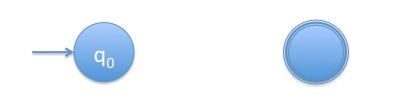
\includegraphics[max width=\textwidth]{:lfa:emptyset.jpg}
\end{figure}


It is clear that this automaton accepts no word, and obeys the three aforementioned conditions.

\textbf{Basis case $E=\epsilon$}

We construct the following automaton:

\begin{figure}[!htb]
\centering
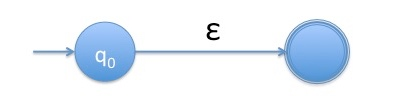
\includegraphics[max width=\textwidth]{:lfa:emptyword.jpg}
\end{figure}


hich only accepts the empty word.

\textbf{Basis case $E=c$} where $c$ is a symbol of the alphabet.

We construct the following automaton:


\begin{figure}[!htb]
\centering
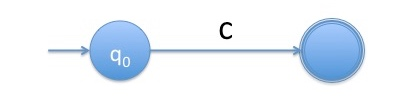
\includegraphics[max width=\textwidth]{:lfa:char.jpg}
\end{figure}


Since regular expressions have three \textit{inductive rules} for constructing regular expressions (union, concatenation and Kleene-star), we have to treat three induction steps:

\textbf{Induction step $E=E_1E_2$ (concatenation)}

Suppose $E_1$ and $E_2$ are regular expressions for which NFAs can be built (\textbf{induction hypothesis}). We build the following NFA which accepts all words generated by the regular expression $E_1E_2$.


\begin{figure}[!htb]
\centering
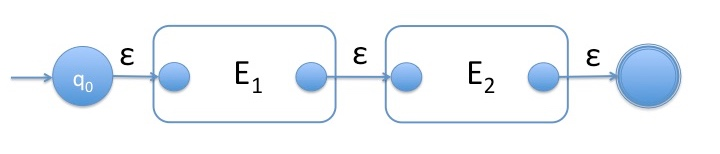
\includegraphics[max width=\textwidth]{:lfa:concat.jpg}
\end{figure}



\textbf{Induction step $E=E_1\cup E_2$ (union)}

Suppose $E_1$ and $E_2$ are regular expressions for which NFAs can be built (\textbf{induction hypothesis}). We build the following NFA which accepts all words generated by the regular expression $E_1\cup E_2$.


\begin{figure}[!htb]
\centering
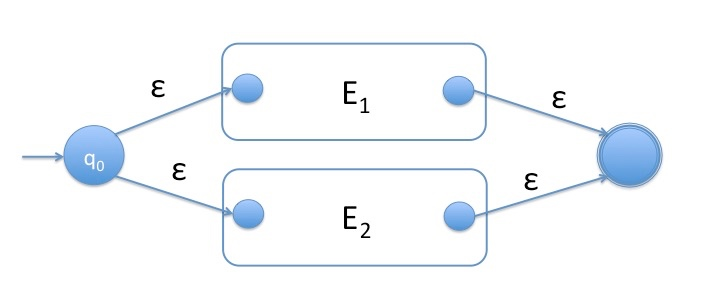
\includegraphics[max width=\textwidth]{:lfa:union.jpg}
\end{figure}


\textbf{Induction step $E^*$ (union)}

Suppose $E$ is regular expression for which an NFA can be built (\textbf{induction hypothesis}). We build the following NFA which accepts all words generated by the regular expression $E*$.


\begin{figure}[!htb]
\centering
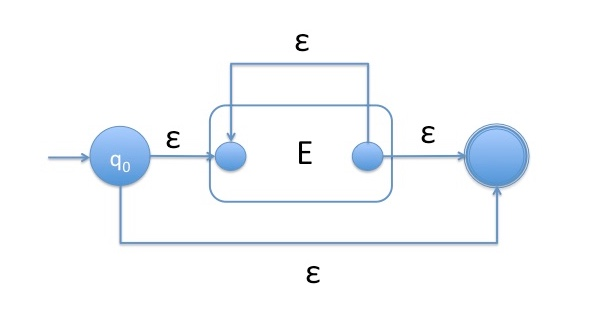
\includegraphics[max width=\textwidth]{:lfa:kleene.jpg}
\end{figure}



\end{proof}

We illustrate the algorithmic procedure on our regular expression $(A\cup B)(a\cup b)*(0 \cup 1)*$.
The result is shown below:


\begin{figure}[!htb]
\centering
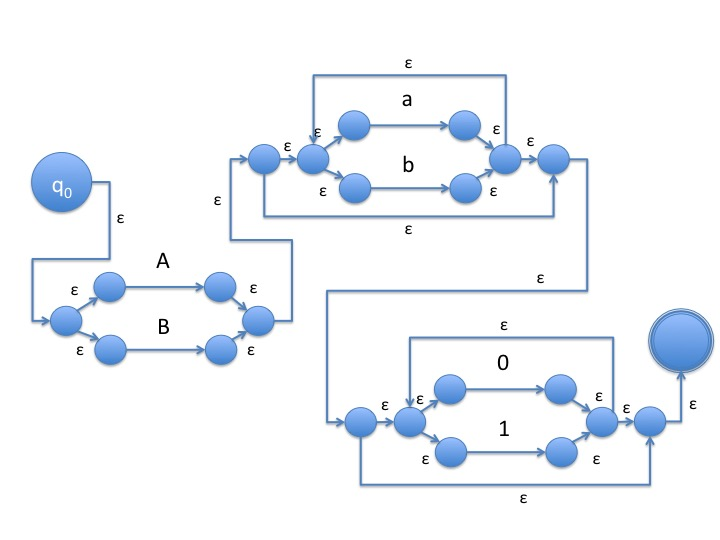
\includegraphics[max width=\textwidth]{:lfa:slide4.jpg}
\end{figure}





\end{document}